%% Default Latex document template
%%
%%  blake@rcs.ee.washington.edu

\documentclass[letterpaper]{article}

% Uncomment for bibliog.
%\bibliographystyle{unsrt}

\usepackage{graphicx}
\usepackage{lineno}
\usepackage{hyperref}
%\usepackage{fancyhdr}

%%%%%%%%%%%%%%%%%%%%%%%%%%%%%%%%%%%%%%%%5
%
%  Set Up Margins

%%%%%%%%%%%%%%%%%%%%%%%%%%%%%%%%%%%%%%%%%%%%%%%%%
% include file for:
%      Critical Page setup dimensions
%            DO NOT MODIFY
%       (for help see "Latex Line by Line" p 260)
%
\setlength\oddsidemargin{0in}
\setlength\evensidemargin{0in}

\usepackage[left=0.98in, right=0.98in, top=1.0in, bottom=1.0in]{geometry}

% %Top Margin and header
% \setlength\voffset{-0.94in}
% \setlength\topmargin{0.25in}
% \setlength\headheight{0.25in}
% %\setlength\headwidth{6.5in}
% \setlength\headsep{0.25in}
% %Body
% \setlength\textwidth{6.5in}
% \setlength\textheight{9.50in}
% %Footer
% %\setlength\footheight{0.5in}
% \setlength\footskip{0.3750in}
% Line spacing for 6 lines per inch
\linespread{0.894}  % 1.0 = single    1.6 = double
%
%          END of Critical Page Setup Dimensions
%%%%%%%%%%%%%%%%%%%%%%%%%%%%%%%%%%%%%%%%%%%%%%%%%%%

%%%%%%%%%%%%%%%%%%%%%%%%%%%%%%%%%%%%%%%%%%%%%%%%%%%
%
% Useful style and math macros
%


\newcommand\Dfrac[2]{\frac{\displaystyle #1}{\displaystyle #2}}
\newcommand\beq{\begin{equation}}
\newcommand\eeq{\end{equation}}

\newcommand\bmat{\begin{bmatrix}}
\newcommand\emat{\end{bmatrix}}

\newenvironment{solution}
{\ttfamily \vspace{0.155in} {\bf SOLUTION:} \\ }
{ \vspace{0.25in} \par }



%
%        Font selection
%
%\renewcommand{\rmdefault}{ptm}             % Times
%\renewcommand{\rmdefault}{phv}             % Helvetica
%\renewcommand{\rmdefault}{pcr}             % Courier
%\renewcommand{\rmdefault}{pbk}             % Bookman
%\renewcommand{\rmdefault}{pag}             % Avant Garde
%\renewcommand{\rmdefault}{ppl}             % Palatino
%\renewcommand{\rmdefault}{pch}             % Charter


%%%%%%%%%%%%%%%%%%%%%%%%%%%%%%%%%%%%%%%%%%%%%%%%%
%
%         Page format Mods HERE
%
%Mod's to page size for this document
\addtolength\textwidth{0cm}
\addtolength\oddsidemargin{0cm}
\addtolength\headsep{0cm}
\addtolength\textheight{0cm}
%\linespread{0.894}   % 0.894 = 6 lines per inch, 1 = "single",  1.6 = "double"

% header options for fancyhdr

%\pagestyle{fancy}
%\lhead{LEFT HEADER}
%\chead{CENTER HEADER}
%\rhead{RIGHT HEADER}
%\lfoot{Hannaford, U. of Washington}
%\rfoot{\today}
%\cfoot{\thepage}



% Make table rows deeper
%\renewcommand\arraystretch{2.0}% Vertical Row size, 1.0 is for standard spacing)

\begin{document}
\setpagewiselinenumbers        %  Line numbers for edits to drafts.
\modulolinenumbers[1]          %  number every N lines

% \linenumbers                   %  start numbering lines here


\date{\today}

\section*{4x4 State Transition Criteria}
First we define Drive pressure, $drivepress,$
as the pressure in the compartment which drives eversion.
This is compartment 1 for the 1-compartment model and compartment 2 for the 2-compartment
model.  We also define
$L_c$, the length of material in the crumple zone between reel and everting
portion as,
\beq
L_c = \theta r_{reel} - 2L
\eeq

We then test some state variables to determine four boolean
state transition  conditions:
\begin{verbatim}
        LoPress = drivepress < Pth1
        HiPress = drivepress > Pth2
        SlackExists = Lc > epsilon
        noSlack =  Lc < epsilon
\end{verbatim}

\texttt{LoPress} and \texttt{HiPress} determine when the eversion process stops and starts
respectively. \texttt{SlackExists} and \texttt{noSlack} define conditions for when
material crumples inside the housing between the reel and the eversion tube.

We then construct a table determining all transitions between the four possible states
(Table \ref{4x4stateTable}).


\begin{table}[h]
\begin{tabular}{c|c|c|c|c}
 To: \\From: &  Growing-Taut   & Growing-Slack   & Stuck-Taut  & Stuck-Slack \\ \hline
             &     0  & 1 & 2 & 3 \\ \hline
0    &  & SlackExists & LoPress  & LoPress {\bf and} SlackExists \\ \hline
1    & noSlack  &   & LoPress \textbf{and} noSlack  &  LoPress \\ \hline
2    & HiPress    & HiPress \textbf{and} SlackExists &   &  SlackExists \\ \hline
3    & HiPress \textbf{and} noSlack & HiPress &   & \\
\end{tabular}\caption{4x4 state transition diagram deterimining growing or stuck and
taut or slack substates.  State in each row makes transitions to
column state when conditions
in each cell are met. Blank cells indicating in the same state.}\label{4x4stateTable}
\end{table}


These state transitions are illustrated diagrammatically in Figure \ref{4x4StateDiagram}.

\begin{figure}[h]\centering
        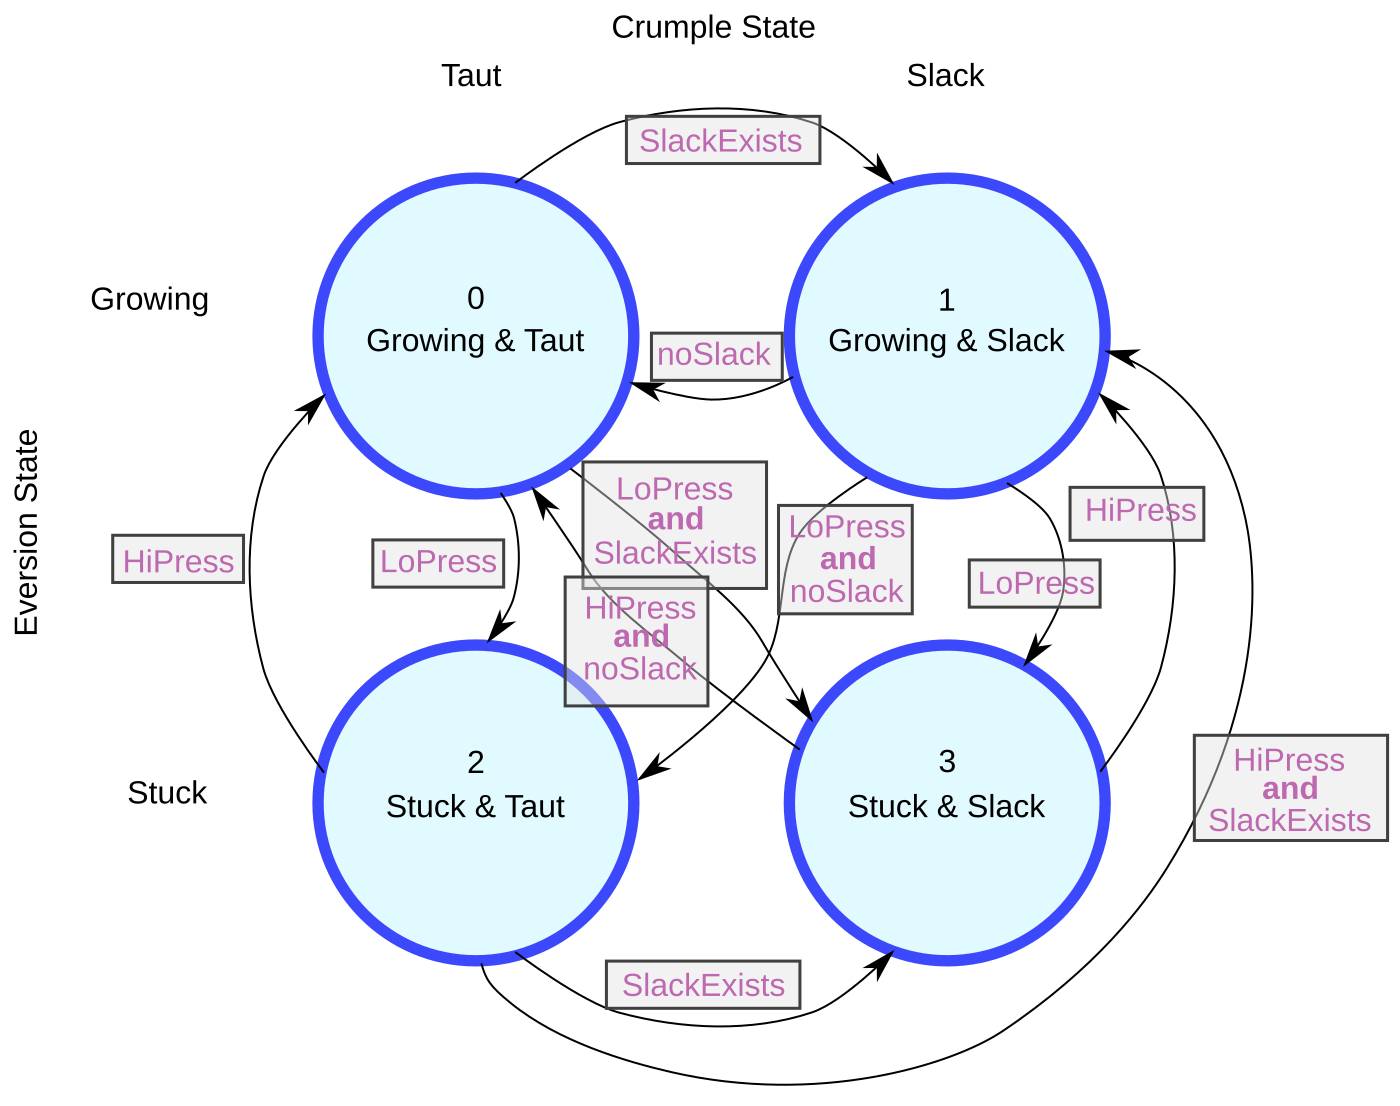
\includegraphics[width=0.5\textwidth]{4x4StateTransDiag.png}
        \caption{}\label{4x4StateDiagram}
\end{figure}



%  Use name of bibliography files without .bib extension
%\bibliography{brl}



\section{Tubing Resistance}


\begin{figure}
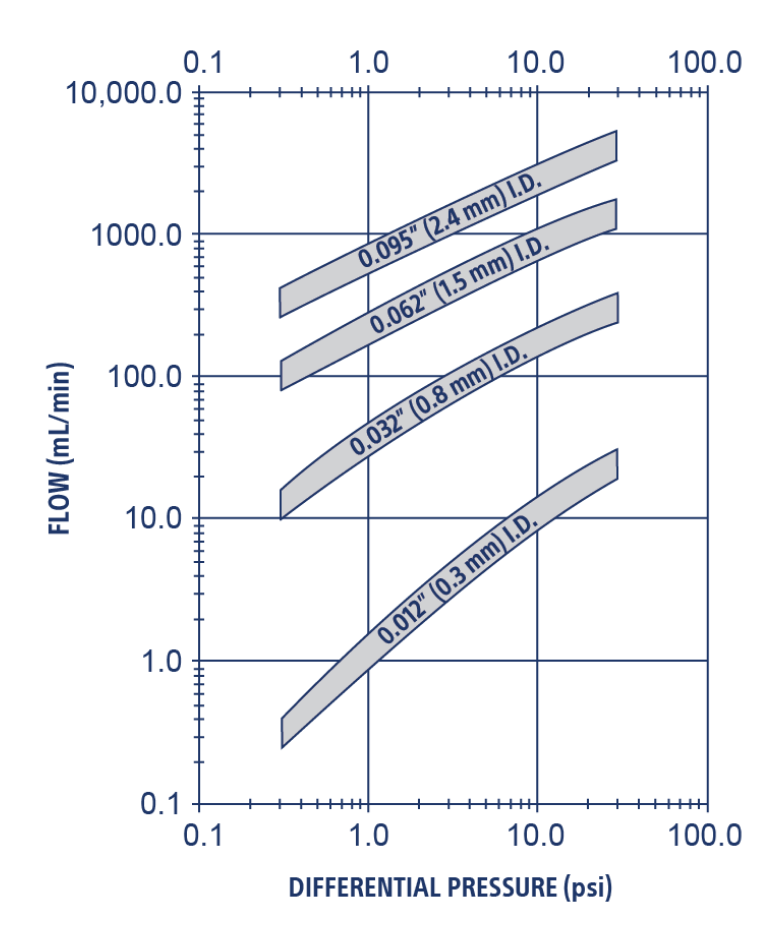
\includegraphics[width=0.5\textwidth]{TubingResChart.png}
\caption{source: The Lee Company  \\ \url{https://www.theleeco.com/support-resources/engineering-tools/reference-information/tubing-flow/}}
\end{figure}



\end{document}

